
\documentclass{acm_proc_article-sp}


\begin{document}

\title{Linked Data-driven Web Components}
\subtitle{}

\numberofauthors{1} %  in this sample file, there are a *total*
\author{
% 1st. author
\alignauthor
Ali Khalili\\
       \affaddr{Dept. of Computer Science}\\
       \affaddr{VU University Amsterdam}\\
       \affaddr{The Netherlands}\\
       \email{a.khalili@vu.nl}
}


\maketitle
\begin{abstract}
This paper provides a ...

\end{abstract}


\section{Introduction}
The


The remainder of this article...

\section{Related Work}

\section{Web Components}
\emph{Web Components} are a set of W3C standards that enable the creation of reusable widgets or components in Web documents and Web applications.
Web components aim to bring \emph{Component-Based Software Development} (CBSD) to the World Wide Web.

\section{Linked Data-riven Web Components}

Definition



\subsection{Features}

Fine-grained Web applications

\begin{figure}[tb]
  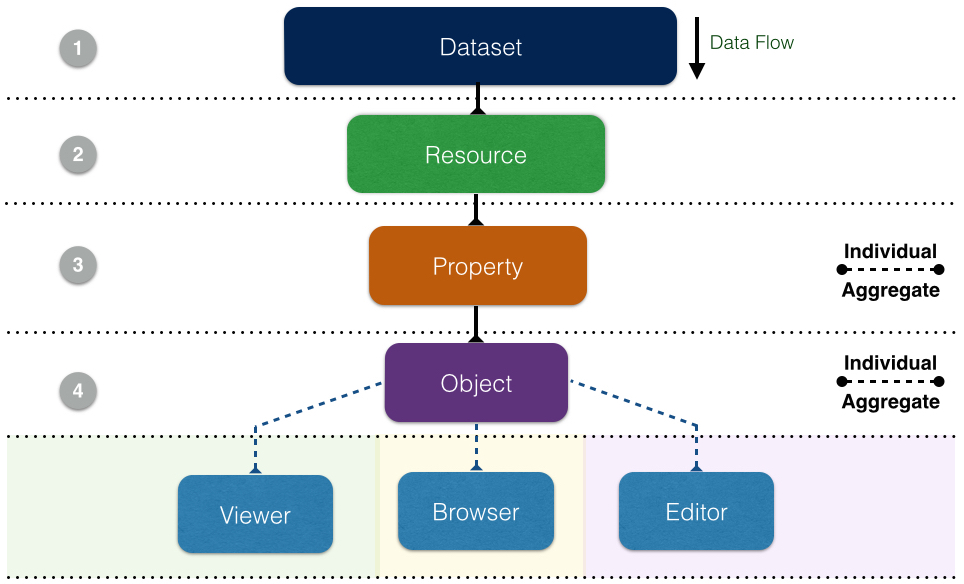
\includegraphics[width=.9\linewidth]{images/architecture.jpg}
  \caption{Architecture}
\end{figure}

- component architecture

- access control

\begin{figure}[tb]
  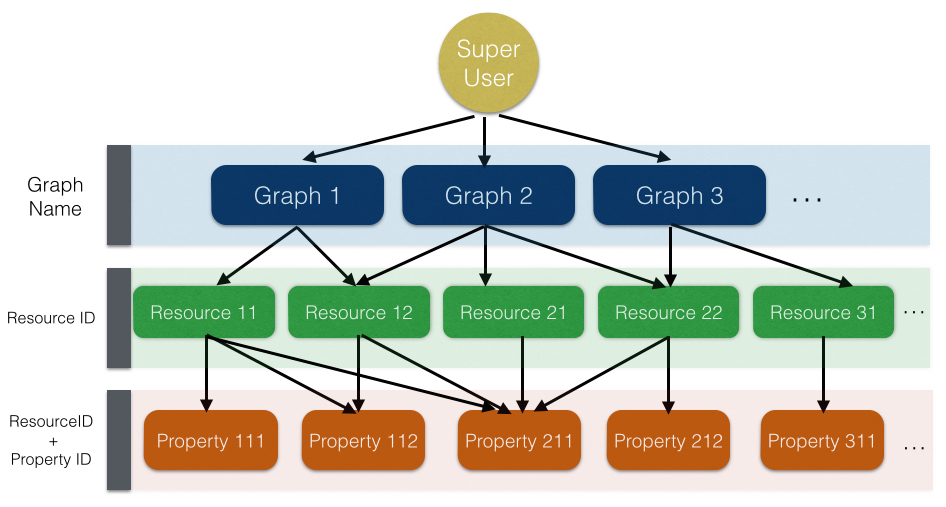
\includegraphics[width=.9\linewidth]{images/userAccessLevels.jpg}
  \caption{User Access Levels}
\end{figure}


Customization and Personalization

- scopes

\begin{figure}[tb]
  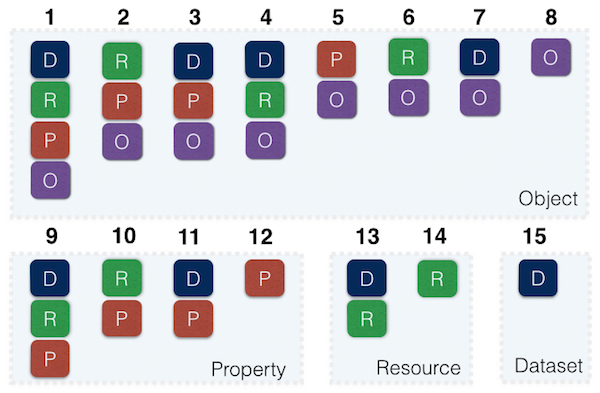
\includegraphics[width=.9\linewidth]{images/scopes.jpg}
  \caption{Scopes}
\end{figure}

Better content visibility reusability

- RDFa, Microdata

Better component visibility, reusability and assembly


\subsection{Life Cycle}

\begin{figure}[tb]
  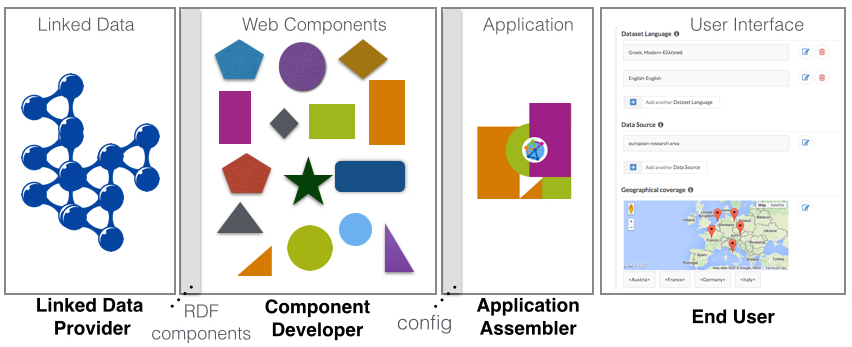
\includegraphics[width=1\linewidth]{images/lifecycle.jpg}
  \caption{Life-cycle}
\end{figure}

\section{Implementation}

http://ld-r.org


\begin{figure}[tb]
  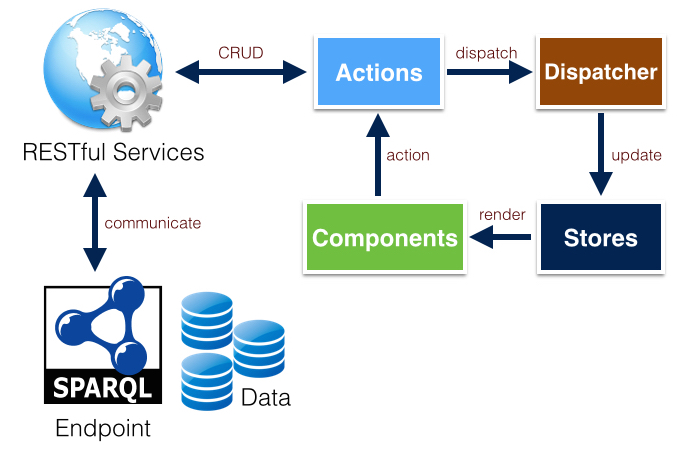
\includegraphics[width=.9\linewidth]{images/dataflow.jpg}
  \caption{Data Flow}
\end{figure}

\begin{figure}[tb]
  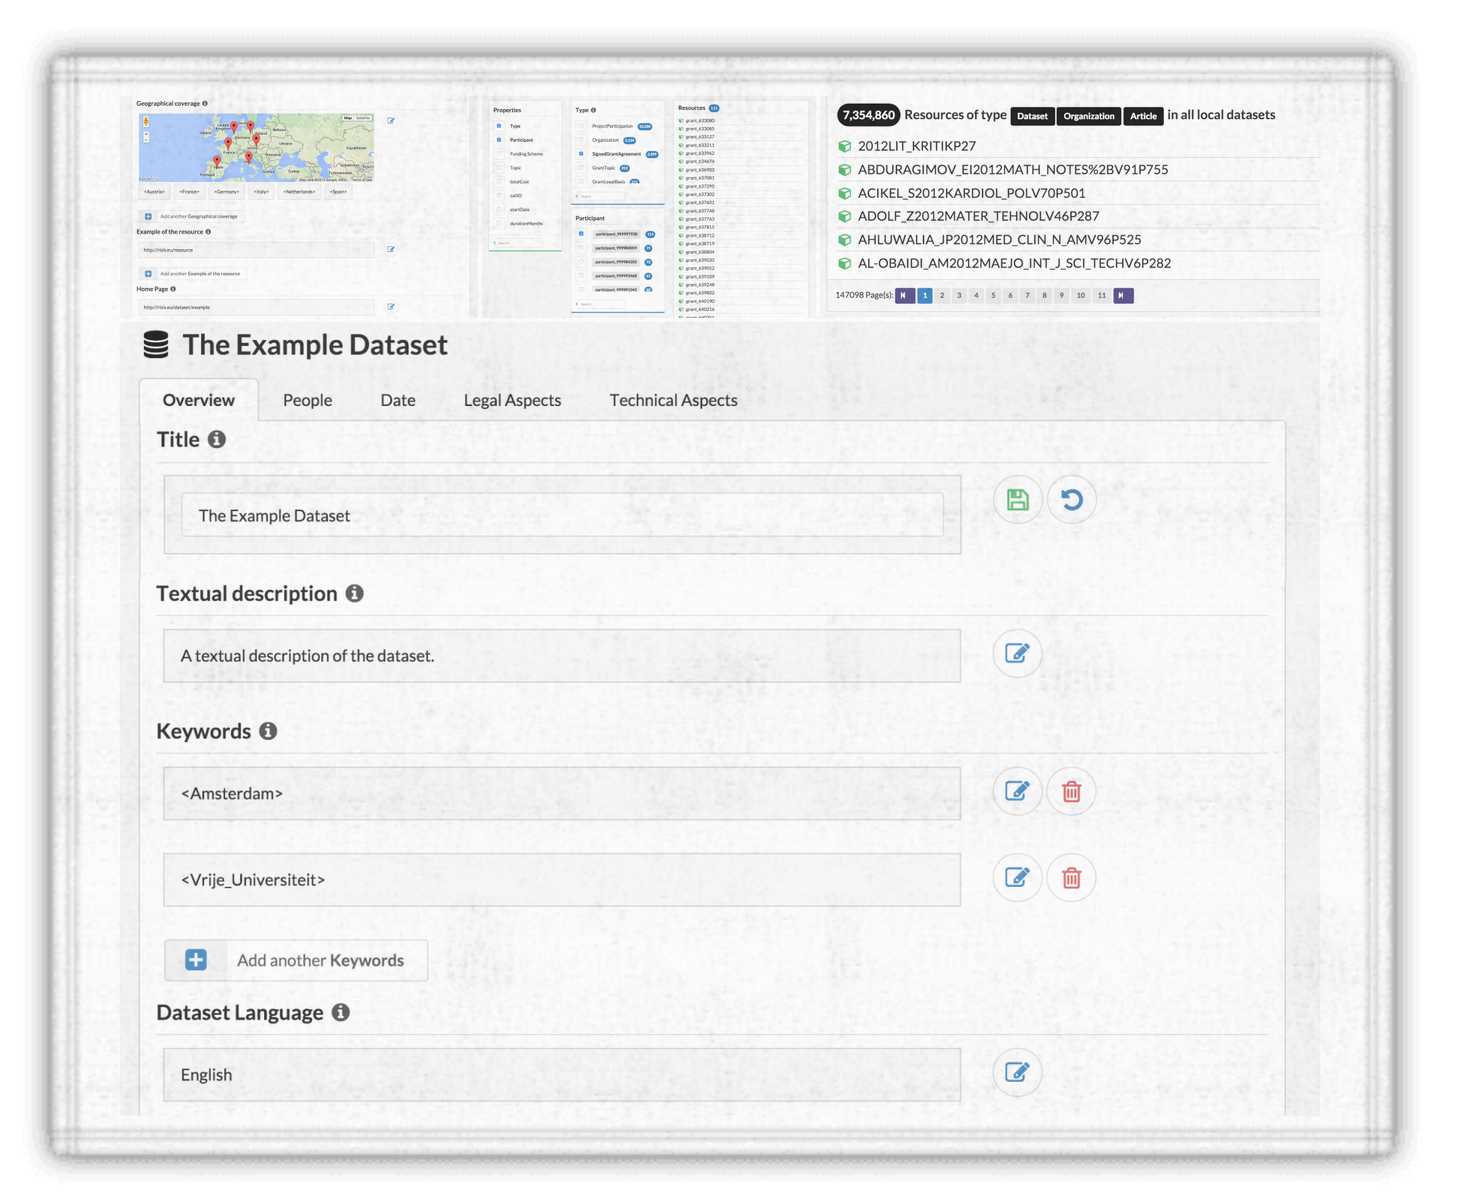
\includegraphics[width=.9\linewidth]{images/screenshot.png}
  \caption{Screenshot}
\end{figure}

\section{Evaluation}

RISIS

OpenPhacts

\section{Conclusion and Future Work}

\section{Aknowledgement}
We would like to thank our colleagues from the KRR research group at VU University Amsterdam for their helpful comments during the development of the LD-R framework. This work was supported by a grant from the European Union’s 7th Framework Programme provided for the project RISIS (GA no. 313082).

\section{References}
\end{document}
